\documentclass[12pt,letterpaper]{article}
\usepackage[utf8]{inputenc}
\usepackage{listings, float, xcolor}

%----- Configuración del estilo del documento------%
\usepackage{graphicx, fancyhdr}
\usepackage{enumitem, pifont, hyperref, ulem, tabularx}
\usepackage[left=2cm,right=2cm,top=1.8cm,bottom=2.3cm]{geometry}


%------ Paquetes matemáticos básicos --------%
\usepackage{amsmath, amssymb, amsthm}

\renewcommand{\lstlistingname}{Código}

%------ Definimos los colores para la sintaxis del código --------%
\definecolor{keywordcolor}{rgb}{0.5, 0.0, 0.5}  % Morado para palabras clave
\definecolor{commentcolor}{rgb}{0.25, 0.5, 0.35} % Verde para comentarios
\definecolor{stringcolor}{rgb}{0.88, 0.68, 0.18}  % Mostaza anaranjado para los strings
\definecolor{backgroundcolor}{rgb}{0.95, 0.95, 0.95} % Gris claro para fondo

%------ Configuración para mostrar código en C++ --------%
\lstdefinestyle{cppstyle}{
  language=C++,
  basicstyle=\ttfamily\footnotesize,
  keywordstyle=\color{keywordcolor}\bfseries,
  commentstyle=\color{commentcolor},
  stringstyle=\color{stringcolor},
  numbers=left,
  numberstyle=\tiny,
  stepnumber=1,
  numbersep=8pt,
  backgroundcolor=\color{backgroundcolor},
  tabsize=2,
  showspaces=false,
  showstringspaces=false,
  breaklines=true,
  frame=single,
  captionpos=b
}

\begin{document}

%------ Encabezado -------- %
\hrule height 0.1pt
\bigskip
\begin{center}
  \begin{minipage}{3cm}
    \begin{center}
      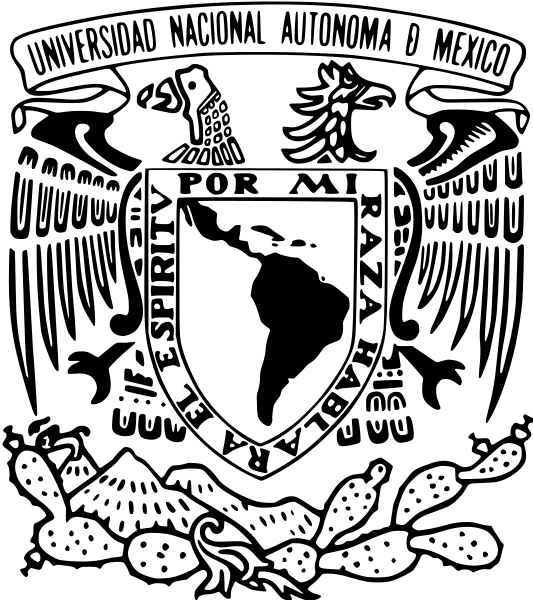
\includegraphics[height=3.4cm]{../unam_logo.png}
    \end{center}
  \end{minipage}\hfill
  \begin{minipage}{10cm}
    \begin{center}
      \textbf{\Large Universidad Nacional Autónoma de México}\\[0.2cm]
      \textbf{\large Facultad de Ciencias}\\[0.2cm]
      \textbf{Organización y Arquitectura de Computadoras 2025-2}\\[0.4cm]
      \textbf{\Large Práctica 09}\\[0.1cm]
      \textbf{Docentes:}\\
      José Galaviz \hspace{1em} Ricardo Pérez \hspace{1em} Ximena Lezama\\[0.3cm]
      \textbf{Autores:}\\
      Fernanda Ramírez Juárez \quad Ianluck Rojo Peña\\[0.3cm]
      \textbf{Fecha de entrega:} Jueves 9 de abril de 2026
    \end{center}
  \end{minipage}\hfill
  \begin{minipage}{3cm}
    \begin{center}
      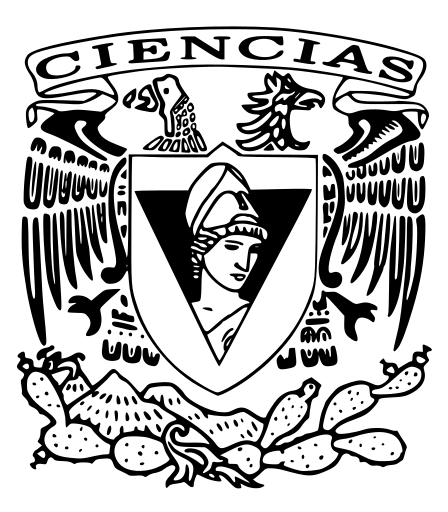
\includegraphics[height=3.4cm]{../fc_logo.png}
    \end{center}
  \end{minipage}
\end{center}

\bigskip
\hrule height 0.1pt
\bigskip

%------ Contenido -------- %
\section*{Preguntas.}

\begin{enumerate}
\item En las llamadas a sistema, las bibliotecas y APIs funcionan como intermediario entre el usuario y las llamadas a sistema. ¿Qué bibliotecas contienen esas llamadas a sistema en Unix y en Windows? ¿Que llamadas al sistema están contenidas en esos archivos?
  % -- Respuesta -- %
  
  \medskip
  
  En sistemas operativos, las bibliotecas y APIs actúan como intermediarios entre las aplicaciones de usuario; las llamadas al sistema \textit{(system calls)} funciones básicas, de bajo nivel, proporcionadas por el kernel que permiten operaciones como el  manejo de archivos, procesos, memoria y dispositivos.

  \begin{enumerate}[label=\arabic*)]
  \item \textit{\textbf{Unix/Linux}}:
    
    Las llamadas al sistema en Unix/Linux son accesibles a través de bibliotecas estándar que actúan como \textbf{wrappers} \textit{(envoltorios)} para interactuar con el kernel.
    
    \textbf{Bibliotecas principales}.
    \begin{itemize}
      \item \textit{GNU C Library(glibc)}: La implementación estándar más común en Linux. Proporciona funciones como \texttt{open()}, \texttt{fork()} o \texttt{write()}, que finalmente invocan las llamadas al sistema.
      \item \textit{musl libc}: Alternativa ligera a \texttt{glibc}, común en sistemas embebidos o distribuciones minimalistas.    
      \item \textit{libSystem (macOS/BSD)}: En sistemas BSD y macOS, esta biblioteca cumple un rol similar a glibc.       
    \end{itemize}

    \textbf{Ejemplos de llamadas al sistema en Unix/Linux}.
    \begin{itemize}
    \item Archivos: \texttt{open()}, \texttt{read()}, \texttt{write()}, \texttt{close()}.
    \item Procesos: \texttt{fork()}, \texttt{execve()}, \texttt{wait()}, \texttt{exit()}.
    \item Memoria: \texttt{brk()}, \texttt{sbrk()}, \texttt{mmap()}, \texttt{munmap()}.
    \item Redes: \texttt{socket()}, \texttt{bind()}, \texttt{listen()}, \texttt{accept()}.
    \item Dispositivos: \texttt{ioctl()}.
    \end{itemize}

  
  \item \textit{\textbf{Windows}}:

    Windows no expone directamente las llamadas al sistema, sino que ofrece capas de abstracción como la \textbf{WinAPI} y la \textbf{NT API} \textit{(nativa del kernel)}.

    \textbf{Bibliotecas principales}.
    \begin{itemize}
      \item \textit{kernel32.dll}: Proporciona funciones de alto nivel para manejo de procesos, memoria y archivos.
      \item \textit{ntdll.dll}: Interfaz entre las llamadas de WinAPI y las llamadas nativas del kernel \textit{(NT API)}. Contiene wrappers como NtCreateFile.
      \item Otras DLLs: \textit{user32.dll} (interfaz gráfica), \textit{ws2\_32.dll} (redes).
    \end{itemize}

    \textbf{Ejemplos de llamadas equivalentes en Windows}.
    \begin{itemize}
      \item Archivos: \texttt{CreateFile()}, \texttt{ReadFile()}, \texttt{WriteFile()}, \texttt{CloseHandle()}.
      \item Procesos: \texttt{CreateProcess()}, \texttt{ExitProcess()}, \texttt{WaitForSingleObject()}.
      \item Memoria: \texttt{VirtualAlloc()}, \texttt{VirtualFree()}.
      \item Redes: \texttt{WSASocket()}, \texttt{Connect()}, \texttt{Send()}.
    \end{itemize}
    
    Las llamadas nativas del kernel \textit{(NT API)} tienen prefijo Nt ejemplo: \textbf{NtCreateFile}, pero no están documentadas oficialmente por Microsoft. Se accede a ellas indirectamente a través de \textbf{ntdll.dll}.
  \end{enumerate}
  
  \bigskip
  
\item Describe que causa, que llamada a sistema y que es o que hacen las siguientes vulnerabilidades a Sistema causadas por la llamadas a Sistema en Linux (registradas con los sufijos CVE):
  \begin{itemize}
  \item Dirty Cow
  \item Dirty Pipe
  \item Baron Samedit Sudo
  \item Residual Risk Flaw
  \end{itemize}
  % -- Respuesta -- %

  \textbf{Vulnerabilidades en Linux relacionadas con llamadas al sistema (CVE)}.
  
  \begin{enumerate}[label=\arabic*)]
  \item \textbf{\textit{Dirty COW (CVE-2016-5195)}}.
    \begin{itemize}
    \item Su causa de debe a la condición de carrera \textit{(race condition)} en el mecanismo \textbf{Copy-On-Write} \textit{(COW)} del kernel al manejar mapeos de memoria privada.
      
    \item Permite a un usuario sin privilegios modificar archivos solo lectura (incluyendo binarios SUID o archivos del sistema).
      
    \item Llamadas al sistema involucradas:
      \begin{itemize}
        \item \texttt{mmap()}: Para mapear memoria.
        \item \texttt{write()}: Intento de escritura en memoria mapeada.
      \end{itemize}
      Fallo clave: El kernel no sincronizaba correctamente hilos al actualizar páginas COW.
      
    \item Impacto:
      \begin{itemize}
        \item Elevación de privilegios local \textit{(Local Privilege Escalation, LPE)} que es un tipo de ataque donde un usuario sin permisos administrativos logra aumentar sus privilegios dentro del sistema.
        \item Ejemplo: modificar /etc/passwd o ganar acceso root.
      \end{itemize}
      Parcheado en \textbf{Linux 4.8.3} (2016).
    \end{itemize}

    
  \item \textbf{\textit{Dirty Pipe (CVE-2022-0847)}}.
    \begin{itemize}
    \item Su causa es el error en el manejo de pipes y la caché de páginas del kernel. Aprovecha una condición de carrera en splice() para escribir en archivos de solo lectura.

    \item Llamadas al sistema involucradas:
      \begin{itemize}
      \item \texttt{splice()}: Transfiere datos entre pipes y archivos sin copiar a user-space.
      \end{itemize}
      Fallo clave: El kernel no validaba permisos al escribir en caché de páginas compartidas.
      
    \item Impacto:
      \begin{itemize}
      \item Sobrescritura de archivos críticos \textit{(ejecutables SUID, configuraciones del sistema)}.
      \end{itemize}
      Afectó kernels \textbf{5.8} a \textbf{5.16.11} (parcheado en 2022).
    \end{itemize}
    
  \item \textbf{\textit{Baron Samedit (CVE-2021-3156, Sudo)}}.
    \begin{itemize}
    \item Su causa es el desbordamiento de búfer \textit{(heap-based overflow)} en \texttt{sudoedit} al procesar argumentos malformados en modo no-interactivo.
      
    \item Llamadas al sistema involucradas:
      \begin{itemize}
      \item \texttt{execve()}: Para ejecutar \texttt{sudoedit}.
      \end{itemize}
      No es un fallo del kernel, sino del manejo de memoria en espacio de usuario (sudo).
      
    \item Impacto:
      \begin{itemize}
      \item Elevación a root sin contraseña.
      \end{itemize}
      Afectó a Sudo antes de la versión \textbf{1.9.5p2} (2021).
    \end{itemize}

  \item \textbf{\textit{Residual Risk}}.
    \begin{itemize}
    \item No es una vulnerabilidad específica, sino un concepto de seguridad que refiere a riesgos remanentes tras aplicar controles. Puede involucrar llamadas al sistema si hay permisos mal configurados, ejemplos servicios que no dropean privilegios.
      
    \item Relación con llamadas al sistema:
      \begin{itemize}
      \item Cualquier llamada mal gestionada.
      \item Ejemplo: \texttt{open()}, \texttt{chmod()} puede dejar riesgos residuales.
      \end{itemize}
      
    \item Impacto:
      \begin{itemize}
      \item Depende de la implementación.
      \item Ejemplo: ejecución de código con privilegios no revocados.
      \end{itemize}
    \end{itemize}
    
  \item \textbf{\textit{Flaw (Término genérico)}}.
    \begin{itemize}
    \item Su causa es el error genérico en el kernel o programas (no específico). Como bugs en manejo de hilos (\texttt{clone()}), drivers (\texttt{ioctl()}), etc.
      
    \item Llamadas al sistema involucradas:
      \begin{itemize}
      \item Depende del fallo.
      \item Ejemplo: \texttt{ioctl()} para drivers, \texttt{clone()} para hilos.
      \end{itemize}
      
    \item Impacto:
      Desde denegación de servicio (DoS) esto significa que un atacante puede crashar o bloquear un proceso, servicio o incluso todo el sistema, volviéndolo inaccesible o inestable,  hasta ejecución de código arbitrario es decir un atacante puede ejecutar comandos o programas con privilegios elevados.
    \end{itemize}
  \end{enumerate}
\end{enumerate}
\end{document}
